\section{Polymer Diffusion}
In these exercises we want to use the LBM-MD-Hybrid to reproduce a classic
result of polymer physics: The dependence of the diffusion coefficient
of a polymer on its chain length. If no hydrodynamic interactions
are present, one expects a scaling law $D \propto N^{-1}$ and if 
they are present, a scaling law $D \propto N^{-\nu}$ is expected. 
Here $\nu$ is the Flory exponent that plays a very prominent role
in polymer physics. It has a value of $\sim 3/5$ in good solvent
conditions in 3D. Discussions of these scaling laws can be found
in polymer physics textbooks like \cite{degennes79a, doi96a, rubinstein03a}.


The reason for the different scaling law is the following:
When being transported, every monomer creates a flow field that follows
the direction of its motion. This flow field makes it easier 
for other monomers to follow its motion. This makes a polymer
long enough diffuse more like compact object including the fluid
inside it, although it does not have clear boundaries. It can be shown 
that its motion can be described by its hydrodynamic radius. It is defined 
as:
\begin{equation}
  \langle \frac{1}{R_h} \rangle = \langle \frac{1}{N^2}\sum_{i\neq j} \frac{1}{\left| r_i - r_j \right|} \rangle
\end{equation}
This hydrodynamic radius exhibits the scaling law  $R_h \propto N^{\nu}$
and the diffusion coefficient of long polymer is proportional to its inverse.
For shorter polymers there is a transition region. It can be described
by the Kirkwood-Zimm model:
\begin{equation}
  D=\frac{D_0}{N} + \frac{k_B T}{6 \pi \eta } \langle \frac{1}{R_h} \rangle
\end{equation}
Here $D_0$ is the monomer diffusion coefficient and $\eta$ the 
viscosity of the fluid. For a finite system size the second part of the
diffusion is subject of a $1/L$ finite size effect, because
hydrodynamic interactions are proportional to the inverse
distance and thus long ranged. It can be taken into account
by a correction:
\begin{equation}
  D=\frac{D_0}{N} + \frac{k_B T}{6 \pi \eta } \langle \frac{1}{R_h} \rangle \left( 1- \langle\frac{R_h}{L} \rangle \right)
  \label{kirkwood}
\end{equation}
It is quite difficult to prove this formula with good accuracy. It will 
need quite some computer time and a careful analysis. So please don't be
too disappointed if you don't manage to do so.


We want to determine the diffusion coefficient from the mean square
distance that a particle travels in the time $t$. For large $t$ it is
be proportional to the time and the diffusion coefficient occurs as 
prefactor: 
\begin{equation}
  \frac{\partial \langle r^2 \left(t\right)\rangle}{\partial t} = 2 d D. 
  \label{eq:msd}
\end{equation}
Here $d$ denotes the dimensionality of the system, in our case 3.
This equation can be found in virtually any simulation textbook, like
\cite{frenkel02b}.
We will therefore set up a polymer in an LB fluid, simulate for an appropriate
amount of time, calculate the mean square displacement as a function of
time and obtain the diffusion coefficient from a linear fit. However
we make a couple of steps in between and divide the full problem into 
subproblems that allow to (hopefully) fully understand the process.

\subsection{Step 1: Diffusion of a single particle}
Our first step is to investigate the diffusion of a single particle
that is coupled to an LB fluid by the point coupling method.
Take a look at the script \texttt{single\_particle\_diffusion.py}.
The script takes the LB-friction coefficient as an argument. Start with
an friction coefficient of 1.0:
{\vspace{0,2cm}\small
\begin{lstlisting}[numbers=none]
/path/to/pypresso single_particle_diffusion.py 1.0
\end{lstlisting}
\vspace{0,2cm}
}

In this script an LB fluid and a single particle are created and
thermalized. 
The random forces on the particle and
within the LB fluid will cause the particle to move. The mean squared
displacement is calculated during the simulation via a multiple-tau correlator. 
Run the simulation script and plot the output data \texttt{msd\_1.0.dat}. To
load the file into a numpy array, one can use \texttt{numpy.loadtxt}.
Zoom in on the origin of the plot. What do you see for short times? What do you
see on a longer time scale? Produce a double-logarithmic plot to assess the power
law.
\begin{figure}[h]
  \begin{center}
	  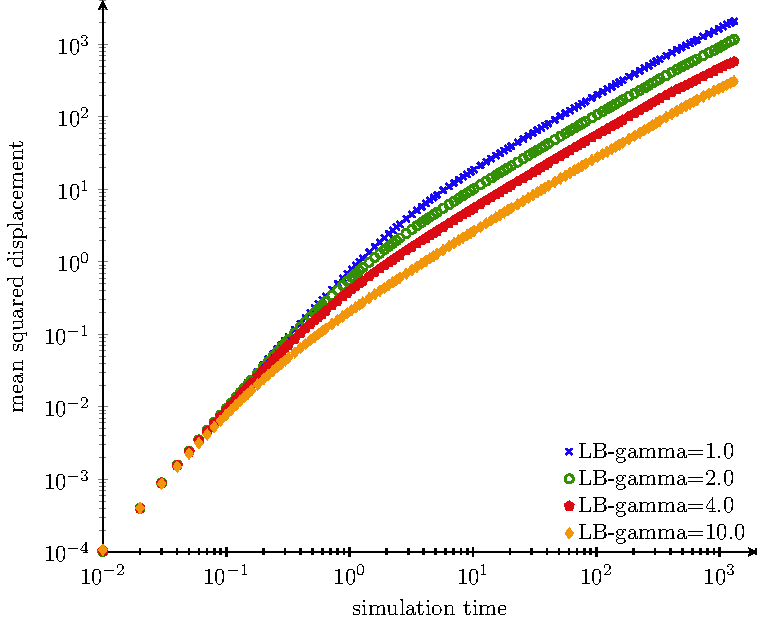
\includegraphics[width=0.7\textwidth]{figures/diffusion/msd.pdf}
  \end{center}
  \caption{Mean squared displacement of a single particle for different values
  of LB friction coefficient.}
\end{figure}

Can you give an explanation for the quadratic time dependency for short
times?
Use the function \texttt{curve\_fit} from the module \texttt{scipy.optimize} to
produce a fit for the linear regime and determine the diffusion coefficient.

%The file \lstinline|energy.dat| contains the kinetic energy of the
%particle as a function of the elapsed simulation time. Investigate
%it, by plotting it with gnuplot. Calculate the average value of 
%the kinetic energy e.g. by fitting a constant function with gnuplot.
%What value would you expect from a working thermostat?

Run the simulation again with different values for the friction
coefficient, e.g. 1. 2. 4. 10. Calculate the diffusion
coefficient for all cases and plot them as a function of $\gamma$. What relation
do you observe?

%The tiny helper script \lstinline|fit_lin.sh| 
%(with argument \lstinline|msd_pos.dat|)
%will help you with that. It contains
%a (quite ugly) gnuplot one-liner that does the fitting and just
%returns the slope. The fit is performed in the range 5 to 40 that
%has proved to work good for runs of $\sim 100000$ steps. You have to 
%modify the script to change that range.
%Is there any difference between the
%friction coefficient that you put in, and the diffusion coefficient
%you obtain?

%\section{Step 3: The long time tail of the velocity autocorrelation function}
%Should we do anything here?

\subsection{Step 2: Diffusion of a polymer}
One of the typical applications of \ES{} is the simulation of polymer chains 
with a bead-spring-model. For this we need a repulsive interaction
between all beads, for which one usually takes a shifted and truncated
Lennard-Jones (so called Weeks-Chandler-Anderson) interaction, 
and additionally a bonded interaction between 
adjacent beads to hold the polymer together.
\pagebreak
 You have already learned
that the command
{\vspace{0,2cm}\small
\begin{pypresso}
  system.non_bonded_inter[0,0].lennard_jones.set_params(
      epsilon = 1.0, sigma = 1.0,
      shift = 0.25, cutof = 1.226)
\end{pypresso}\vspace{0,2cm}
}
creates a Lennard-Jones interaction with $\varepsilon=1.$, $\sigma=1.$,
$r_\text{cut} = 1.125$ and $\varepsilon_\text{shift}=0.25$ between particles
of type 0, which is the desired 
repulsive interaction. The command
{\vspace{0,2cm}\small
\begin{pypresso}
  from espressomd import interactions
  fene = interactions.FeneBond(k = 7,d_r_max = 2)
\end{pypresso}
\vspace{0,2cm}
}
creates a \texttt{FeneBond} object (see \ES{} manual for the details). Still \ES{}
does not know between which beads this interaction should be applied.
This can be either be specified explicitly or done with the \texttt{polymer}
module. This creates a given number of beads, links them with the given
bonded interaction and places them following a certain algorithm. We will
use the pruned self-avoiding walk: The monomers are set according 
to a pruned self-avoiding walk (in 3D) with a
fixed distance between adjacent bead positions. The syntax is:
{\vspace{0,2cm}\small
\begin{pypresso}
  from espressomd import polymer
  # mpc: monomers per chain
  mpc = 30
  poly = polymer.Polymer(N_P=1, MPC = mpc, bond=fene, bond_length = 1)
\end{pypresso}
\vspace{0,2cm}
}
Using a random walk to create a polymer causes trouble: The random walk may 
cross itself (or closely approach itself) and the LJ potential is very
steep. This would raise the potential energy enormously and would make
the monomers shoot through the simulation box. The pruned self-avoiding
walk should prevent that, but to be sure
we perform some MD steps with a capped LJ potential, this means 
forces above a certain threshold will be set to the threshold in order to prevent
the system from exploding. To see how this is done, look at the script 
\texttt{polymer\_diffusion.py}.
It contains a quite long warmup command so that also longer polymers
are possible. You can probably make it shorter.

It is called in the following way:
{\vspace{0,2cm}\small
\begin{lstlisting}[numbers=none]
/path/to/pypresso polymer_diffusion.py $N_monomers  
\end{lstlisting}\vspace{0,2cm}
}
This allows to quickly change the number of monomers without editing 
the script.
For the warmup a Langevin thermostat is used to keep the temperature constant.
Furthermore we want to compute the diffusion constant of the polymer for
different numbers of monomers. For this purpose we can again use the multiple
tau correlator. Have a look at the \ES{} -script for the single particle diffusion
and add the adapted commands for the polymer. Find out how many integration steps are
necessary to capture the long-time diffusion regime of the polymer. The script
already computes the time averaged hydrodynamic radius and stores it in a file
\texttt{rh\_nom\_xx.dat} where \texttt{xx} is the number of monomers.

Run the script for different numbers of monomers and determine the evolution of
the diffusion coefficient as a function of the chain length. Compare the results
of your \ES{} simulations with the given Kirkwood-Zimm formula
(eq.~\ref{kirkwood}). 
